\section{User testing with individual developers}
\label{sec:user-testing}
During my research of the Sensei \gls{ide} plugin, Sensei's product manager at \gls{scw}, Charlie Eriksen, has organized two usability tests.
The first usability test was performed in October 2020, the second several months later in April 2021.
The usability tests were executed by the company Haxor\footnote{\url{https://haxor.sh/}}.
Afterwards, screen recordings and insights were shared with us to evaluate the tests.

\subsection{Goals and research question}
The main \textit{goal} of the tests is to observe developers creating new recipes for the Sensei \gls{ide} plugin.
The \textit{purpose} is evaluating different features of the Sensei recipe editor.
The \textit{quality focus} is the ability of the plugin to allow developers to easily create the recipes they have in mind.
The study evaluates the \gls{ui} and \gls{ux} of the recipe editor.

I aim to observe which features in the recipe editor are most effective and usable.
In the experiment, I evaluated the behaviour of several groups of developers who have a minimum level of expertise in software development in Java.

The above goal can be achieved by means of an experiment aimed at answering the following four questions:
\begin{itemize}
    \item \textbf{Q1} Which features are most useful when creating a recipe?
    \item \textbf{Q2} What are the main shortcomings when creating a recipe?
    \item \textbf{Q3} Which features are most useful when creating a quick-fix?
    \item \textbf{Q4} What are the main shortcomings when creating a quick-fix?
\end{itemize}

The same usability tests are also used by Sensei's product manager to evaluate the installation process, the onboarding process, and the documentation.
Those results will be briefly discussed as well.

\subsection{Experimental set-up}
\subsubsection{Subjects}
For both runs of the experiment, the goal was to have at least five subjects, a frequently used number in usability testing.
It is the number of users needed to detect 85\% of the problems in an interface, given that the probability of each problem occurring is 31\%~\cite{nielsen1993mathematical}.
In practice, \gls{ui} and \gls{ux} problems do not affect users in a predictable way, and the probability that a user encounters a problem can be significantly lower.
In that case a larger number of subjects is needed.
However, it is advised to use an iterative design and test strategy, where five subjects are brought in to find problems and these problems are fixed before bringing in five more~\cite{nielsen1993mathematical}.
In order to guarantee successful tests for five subjects even in the case of a technical problem, each round six subjects were asked to participate.

All subjects are hired by Haxor from the United States and speak English.
They are recruited from the Haxor Developer Community, DevPort, and online freelancing websites.
The subjects are of entry and intermediate skill level and have a minimum of 2 years professional experience.
All of the subjects have programmed in Java before and are familiar with the IntelliJ IDEA.
An effort has been made by Haxor to choose subjects with varying backgrounds, and at least one subject with more than 5 years of professional experience is included in each test.

\subsubsection{Task}
The task was prepared by a \gls{ux} design expert at \gls{scw} in cooperation with the product manager of Sensei and myself.

The developers were given a project with a few fragments of example code.
These code fragments contain various calls to desirable and undesirable methods, made clear through explicit method names, e.g. \texttt{errorTest} and \texttt{completeTest}.

The subjects were tasked to create Sensei recipes and quick-fixes that transform the undesirable method calls into their desirable counterparts.

The required Sensei recipes are of increasing difficulty:

\begin{itemize}[noitemsep]
    \item Recipe 1 is already developed, users are questioned about their understanding of the recipe
    \item Recipe 2 replaces the undesired methodcall by a different methodcall with the same signature (arguments and return type)
    \item Recipe 3 replaces the undesired methodcall by a different methodcall with a different signature (different arguments, same return type)
\end{itemize}

\subsubsection{Experimental procedure}
\paragraph{Testing procedure}
All subjects were allowed to use their own devices, and any resources they would normally use during development, such as books and internet access. To record their session, subjects were instructed to use Paircast\footnote{\url{https://paircast.io/}}.
Paircast is desktop software that records a developer's screen, microphone, code changes, and open applications as they work.

Developers were instructed to speak their thoughts out loud.
In the first round of user testing, the subjects were regularly prompted questions after completing the assigned tasks.
This turned out to be unnecessary as the subject gave plenty feedback without being prompted, hence the questions were dropped in the second round.

I reviewed all of the video recordings.
I manually timed each action, as well as recorded any notable actions or comments made by the subjects.

\subsection{Findings}
\subsubsection{Installation and use}
All of the users who installed the plugin through the Plugins menu and the JetBrains marketplace have done so without any problems and within several minutes.

All users found it easy to understand existing recipes and apply the quick-fixes.
Users claimed the recipes and quick-fixes looked exactly like the IntelliJ quick-fixes and that they would use them frequently.

\subsubsection{Creating recipes and quick-fixes}
When tasked to create new recipes, not all users had as much success, and the opinions were somewhat divided.

The instructions of the first usability test explained that Sensei recipes are stored in a local file called \textit{rules.sensei}.
When reading those instructions, several users opened this file to take a look.
When, in the next steps the users were then prompted to create new recipes, one of them did not look for the recipe editor, but instead began to edit this file at first.
The other users who did find the recipe editor, opened it while the \textit{rules.sensei} file was opened in the text editor.
As a result, the preview panels did not show any relevant code examples.
In the second usability test, the \textit{rules.sensei} file was not mentioned and all users found the recipe editor immediately, and had relevant code files open in the preview panels instead.

In the first usability test, only one user was able to find Sensei documentation by searching for it on the internet, 3 of the other users asked for more documentation when they could not find any.
For the second test, the documentation was easier to find, and all of the users looked for it and found it.
Some users in both tests took their time to read the documentation, they followed along with the getting started guide, for example.
All of these users reported they found it easy to create new recipes.
The users who opened existing recipes in the recipe editor before trying to make their own, generally had less difficulties creating new recipes than users who did not look at examples.

Many users used the context menu to open the recipe editor.
However, in the context menu all of the users selected the option ``start from scratch".
For some users this was because their caret was not in a relevant position, others simply did not use the context-aware options when given the opportunity.
It is possible that the different options in the context menu need to be more descriptive.

When creating a new recipe in the recipe editor, some users were overwhelmed by the code view, all of them preferred to use the \gls{ui} view.
One user refused to create a new recipe, saying they do not want to learn a new language to do so.

Users who did not look at the documentation closely were more likely to be overwhelmed with the amount of options in the drop-down menus of the recipe editor.
The options to choose from are not clearly enough described, not all users are familiar with the different syntactic components and their differences, e.g. method vs methodcall.
None of the users noticed the hints that describe each of the elements in the drop-down menu when they hover over it, as shown in Figure~\ref{fig:dropdownhint}.

\begin{figure}
  \centering
  %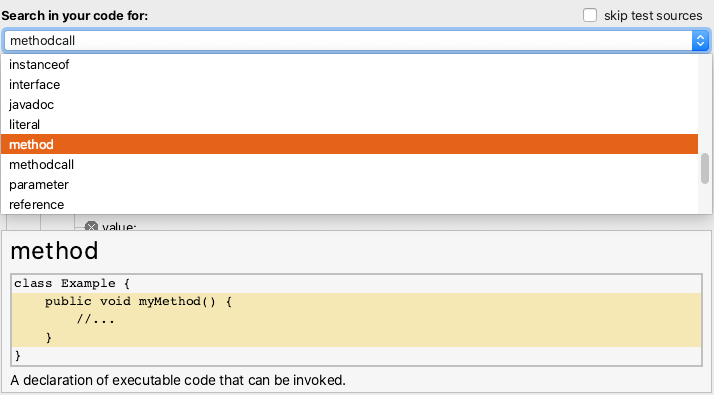
\includegraphics[width=\textwidth]{dropdownhint.png}
  \includegraphics[width=\textwidth,page=6]{04-tools/figures/figures1.pdf}
  \caption[Hints for different syntactic components in the recipe editor]{There are hints available that describe the different syntactic components that can be used in Sensei recipes. These hints are visible when hovering over the different options in the drop-down menu of the recipe editor.}
  \label{fig:dropdownhint} 
\end{figure}

In the fix menu it is possible to reuse arguments of the original code through a template language..
All users who made use of these templates, did so by copying the template from a different recipe and adjusting it to their needs.
None of the users used the suggestions available in the fix menu.

\subsection{Threats to validity}
There are many threats to the validity of conclusions drawn from the findings of these usability tests.
The number of subjects is small and the tasks they were asked to complete are artificial.
The focus of these tests is not to generalize any of the behaviours of the subjects, but rather to identify common usability problems in the interface of the recipe editor.
Several of these problems were detected.
I make no further attempts at interpreting the results from this usability test, I only report the findings as they appeared in the screen recordings.